\documentclass[t]{beamer}
\usepackage{alltt}
\usepackage{verbatim}
\usepackage{graphicx}

\usepackage{tikz}

\newcommand{\bs}{\symbol{`\\}}
\newcommand{\arr}{$\rightarrow$}
\newcommand{\LAMT}[1]{/\bs{}{#1} \arr }
\newcommand{\lam}[1]{\bs{}{#1} \arr }
\newcommand{\oomph}[1]{\textcolor[rgb]{0.0,0.5,0.9}{#1}}
\newcommand{\g}[1]{\textcolor[rgb]{0.7,0.3,0.3}{#1}}
\newcommand{\disab}[1]{\textcolor[rgb]{0.7,0.7,0.7}{#1}}

\begin{document}
\title{SpecConstr: optimising purely functional loops}
\author{Amos Robinson\\PhD student at UNSW}

\frame{\titlepage}

\begin{frame}[fragile]{Compiler divergence}

 Compile this program with \verb/-O2/, and the compiler hangs!

\begin{alltt}
import Data.Vector as V
reverseV = V.foldl (flip (:)) []

> ghc -O2 -v TestReverse.hs
...
*** Simplifier:
Result size of Simplifier
  = {terms: 60, types: 60, coercions: 16}
*** SpecConstr:
Result size of SpecConstr
\end{alltt}
(non termination)

\end{frame}

\begin{frame}[fragile]{Code blowup in stream fusion}
\begin{alltt}
let xs = enumFromTo 1 len
in       (xs ++ xs) `zip` (xs ++ xs)
   `zip` (xs ++ xs) `zip` (xs ++ xs)
   `zip` (xs ++ xs) `zip` (xs ++ xs)

> ghc -O2 -v Blowup.hs
...
*** Simplifier:
Result size of Simplifier
  = {terms: \oomph{678}, types: 2,594, coercions: 9}
*** SpecConstr:
Result size of SpecConstr
  = {terms: \oomph{119,108}, types: 415,625, coercions: 9}
\end{alltt}
(21 seconds)
\end{frame}

\begin{frame}[fragile]{Dot product}
The code we want to write
\begin{alltt}\Large
dotp :: Vector Int -> Vector Int -> Int
dotp as bs
  = fold    (+) 0
  $ zipWith (*) as bs
\end{alltt}
\end{frame}

\begin{frame}[fragile]{Dot product}
The code we want to run
\begin{alltt}\Large
dotp as bs = go 0 0
 where
  go i acc
   | i > V.length as
   = acc
   | otherwise
   = go (i + 1) (acc + (as!i * bs!i))
\end{alltt}
No intermediate vectors, no constructors, no allocations: perfect.

(Just pretend they're not boxed ints...)
\end{frame}

\begin{frame}[fragile]{Dot product}
The code we get after stream fusion (trust me)
\begin{alltt}\Large
dotp as bs = go \oomph{(Nothing,} 0\oomph{)} 0
 where
  go (_, i) acc
   | i > V.length as
   = acc
  go (Nothing, i) acc
   = go (\oomph{Just} (as!i)\oomph{,} i\oomph{)} acc
  go (Just a, i) acc
   = go \oomph{(Nothing,} i + 1\oomph{)} (acc + (a * bs!i))
\end{alltt}
All those allocations!
\end{frame}

\begin{frame}[fragile]{Dot product}
The code we get after stream fusion (trust me)
\begin{alltt}\Large
dotp as bs = go (Nothing, 0) 0
 where
  go \oomph{(}_\oomph{,} i\oomph{)} acc
   | i > V.length as
   = acc
  go \oomph{(Nothing,} i\oomph{)} acc
   = go (Just (as!i), i) acc
  go \oomph{(Just} a\oomph{,} i\oomph{)} acc
   = go (Nothing, i + 1) (acc + (a * bs!i))
\end{alltt}
Only to be unboxed and scrutinised immediately. What a waste!
\end{frame}

\begin{frame}[fragile]{Constructor specialisation}
1. Find all recursive calls in \oomph{go}
\begin{alltt}\Large
dotp as bs = go (Nothing, 0) 0
 where
  go (_, i) acc
   | i > V.length as
   = acc
  go (Nothing, i) acc
   = \oomph{go (Just (as!i), i) acc}
  go (Just a, i) acc
   = \oomph{go (Nothing, i + 1) (acc + (a * bs!i))}
\end{alltt}
So-called interesting call patterns.
\end{frame}

\begin{frame}[fragile]{Constructor specialisation}
2. Create a copy of go for each call pattern
\begin{alltt}
\oomph{go (Nothing, y) z = go'1   y z}
go'1 i acc
 | i > V.length as = acc
 | otherwise       = go (Just (as!i), i) acc

\oomph{go (Just  x, y) z = go'2 x y z}
go'2 a i acc
 | i > V.length as = acc
 | otherwise       = go (Nothing, i + 1) (acc + (a * bs!i))
\end{alltt}
Then find any new call patterns in the new functions' bodies.
\end{frame}

\begin{frame}[fragile]{Constructor specialisation}
3. Apply rewrite rules for each pattern
\begin{alltt}
\oomph{go (Nothing, y) z = go'1   y z}
go'1 i acc
 | i > V.length as = acc
 | otherwise       = \oomph{go'2     (as!i)  i  acc}

\oomph{go (Just  x, y) z = go'2 x y z}
go'2 a i acc
 | i > V.length as = acc
 | otherwise       = \oomph{go'1        (i + 1) (acc + (a * bs!i))}
\end{alltt}
\end{frame}


\begin{frame}[fragile]{After SpecConstr}
Normal optimisation resumes. \oomph{go} is dead.
\begin{alltt}
dotp as bs = go'1 0 0
 where
  \oomph{go (_, i) acc
   | i > V.length as  = acc
  go (Nothing, i) acc = go'2 (as!i) i acc
  go (Just a,  i) acc = go'1 (i + 1) (acc + (a * bs!i))}

  go'1 i acc 
   | i > V.length as  = acc
   | otherwise        = go'2 (as!i) i acc

  go'2 a i acc 
   | i > V.length as  = acc
   | otherwise        = go'1 (i + 1) (acc + (a * bs!i))
\end{alltt}
\end{frame}

\begin{frame}[fragile]{After SpecConstr}
We can inline \oomph{go'2} into \oomph{go'1} and remove the superfluous case.
\begin{alltt}
dotp as bs = go'1 0 0
 where





  go'1 i acc 
   | i > V.length as  = acc
   | otherwise        = \oomph{go'2 (as!i) i acc}

  go'2 a i acc 
   | i > V.length as  = acc
   \oomph{| otherwise        = go'1 (i + 1) (acc + (a * bs!i))}
\end{alltt}
\end{frame}

\begin{frame}[fragile]{After SpecConstr}
And we have the ideal result. 
\begin{alltt}
dotp as bs = go'1 0 0
 where





  go'1 i acc 
   | i > V.length as  = acc
   | otherwise        = \oomph{go'1 (i + 1) (acc + (as!i * bs!i))}
\end{alltt}
\end{frame}


\begin{frame}[fragile]{ForceSpecConstr}
SpecConstr puts a limit on the number of specialisations,
as too many specialisations causes code blowup.
\begin{alltt}
unstream :: Stream a -> [a]
unstream (Stream f s) = go \oomph{ForceSpecConstr} s
 where
  go \oomph{ForceSpecConstr} s
   = case f s of
     Done       -> []
     Skip    s' ->      go \oomph{ForceSpecConstr} s'
     Yield a s' -> a :  go \oomph{ForceSpecConstr} s'
\end{alltt}

But with stream fusion, such as in the \verb/vector/ library, we want to specialise everything no matter what.
\end{frame}

\begin{frame}[fragile]{ForceSpecConstr termination}
A nasty bug in ForceSpecConstr meant that specialising on recursive types would produce infinite specialisations.

\begin{alltt}
reverse :: [a] -> [a]
reverse as = go ForceSpecConstr as []
 where
  go []     acc = acc
  go (a:as) acc = \oomph{go as (a:acc)}

SPECIALISE \oomph{go as (a:acc)}:
go'1 as a acc
 = case as of
    [] -> (a:acc)
    (a':as') -> \oomph{go as' (a':a:acc)}

SPECIALISE \oomph{go as' (a':a:acc)}:
go'2 as' a' a acc
 = ...
\end{alltt}
\end{frame}

\begin{frame}[fragile]{ForceSpecConstr termination}
I fixed this simply by limiting specialisation on recursive types a fixed number of times.

There's a compiler option for this:
\begin{alltt}
>ghc -fspec-constr-recursive=3
\end{alltt}
\end{frame}


\begin{frame}[fragile]{Complicated program}
\begin{alltt}\tiny
-- go = ([0..2] ++ [0..3]) `zip` ([0..3] ++ [0..2])

go :: (Either Int Int, Either Int Int, Maybe Int) -> [Int]
go (Left i, z, Nothing)
 | i <= 2
 = \oomph{go (Left (i+1), z, Just i)}
 | otherwise
 = \oomph{go (Right 0,    z, Nothing)}
go (Right i, z, Nothing)
 | i <= 3
 = \oomph{go (Right (i+1), z, Just i)}
 | otherwise
 = []
go (y, Left  j, Just i)
 | j <= 3
 = (i, z)
 : \oomph{go (y, Left (j+1), Nothing)}
 | otherwise
 = \oomph{go (y, Right 0,    Nothing)}
go (y, Right j, Just i)
 | j <= 2
 = (i, z)
 : \oomph{go (y, Right (j+1), Nothing)}
 | otherwise
 = []

main = putStrLn $ show $ go (Left 0, Left 0, Nothing)
\end{alltt}
\end{frame}

\begin{frame}{Specialisation graph - 1}
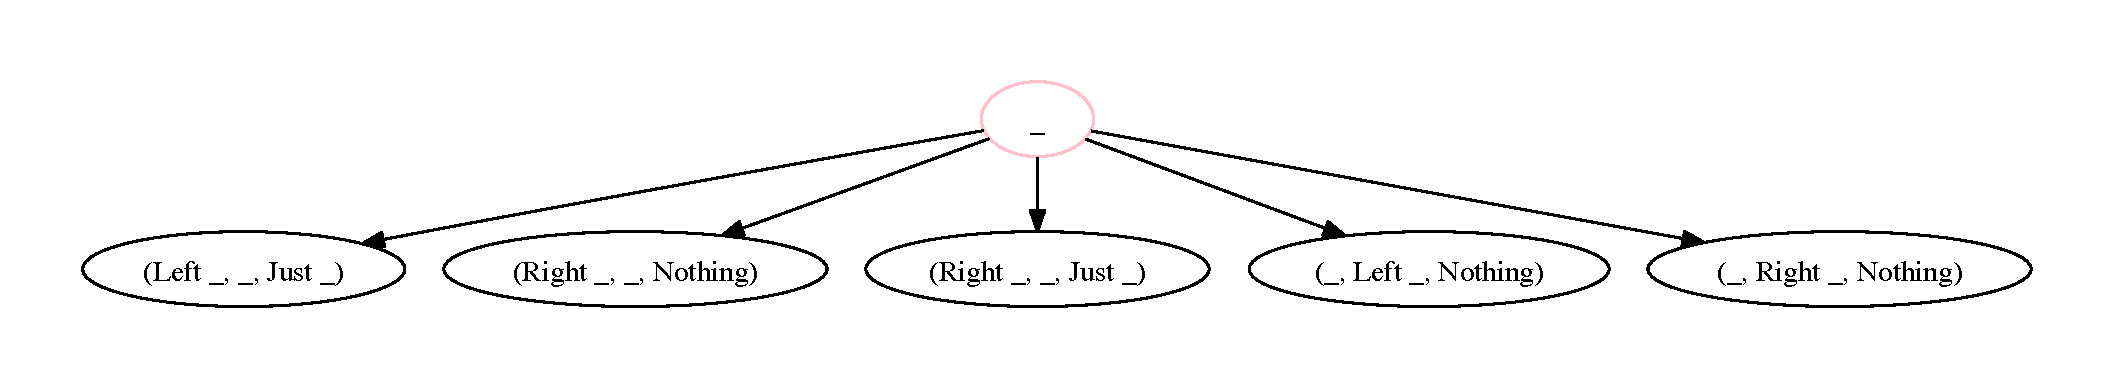
\includegraphics[scale=0.33, trim=10mm 0mm 0mm 10mm, clip]{seeding-1.pdf}
\end{frame}

\begin{frame}[fragile]{Specialisation on (Left \_, \_, Just \_)}
\begin{alltt}\tiny
go :: (Either Int Int, Either Int Int, Maybe Int) -> [Int]
\disab{go (Left i, z, Nothing)
 | i <= 2
 = go (Left (i+1), z, Just i)
 | otherwise
 = go (Right 0,    z, Nothing)
go (Right i, z, Nothing)
 | i <= 3
 = go (Right (i+1), z, Just i)
 | otherwise
 = []}
go (\oomph{Left y}, Left  j, Just i)
 | j <= 3
 = (i, z)
 : \oomph{go (Left y, Left (j+1), Nothing)}
 | otherwise
 = \oomph{go (Left y, Right 0,    Nothing)}
go (\oomph{Left y}, Right j, Just i)
 | j <= 2
 = (i, z)
 : \oomph{go (Left y, Right (j+1), Nothing)}
 | otherwise
 = []
\end{alltt}
\end{frame}

\begin{frame}{Specialisation graph - 2}
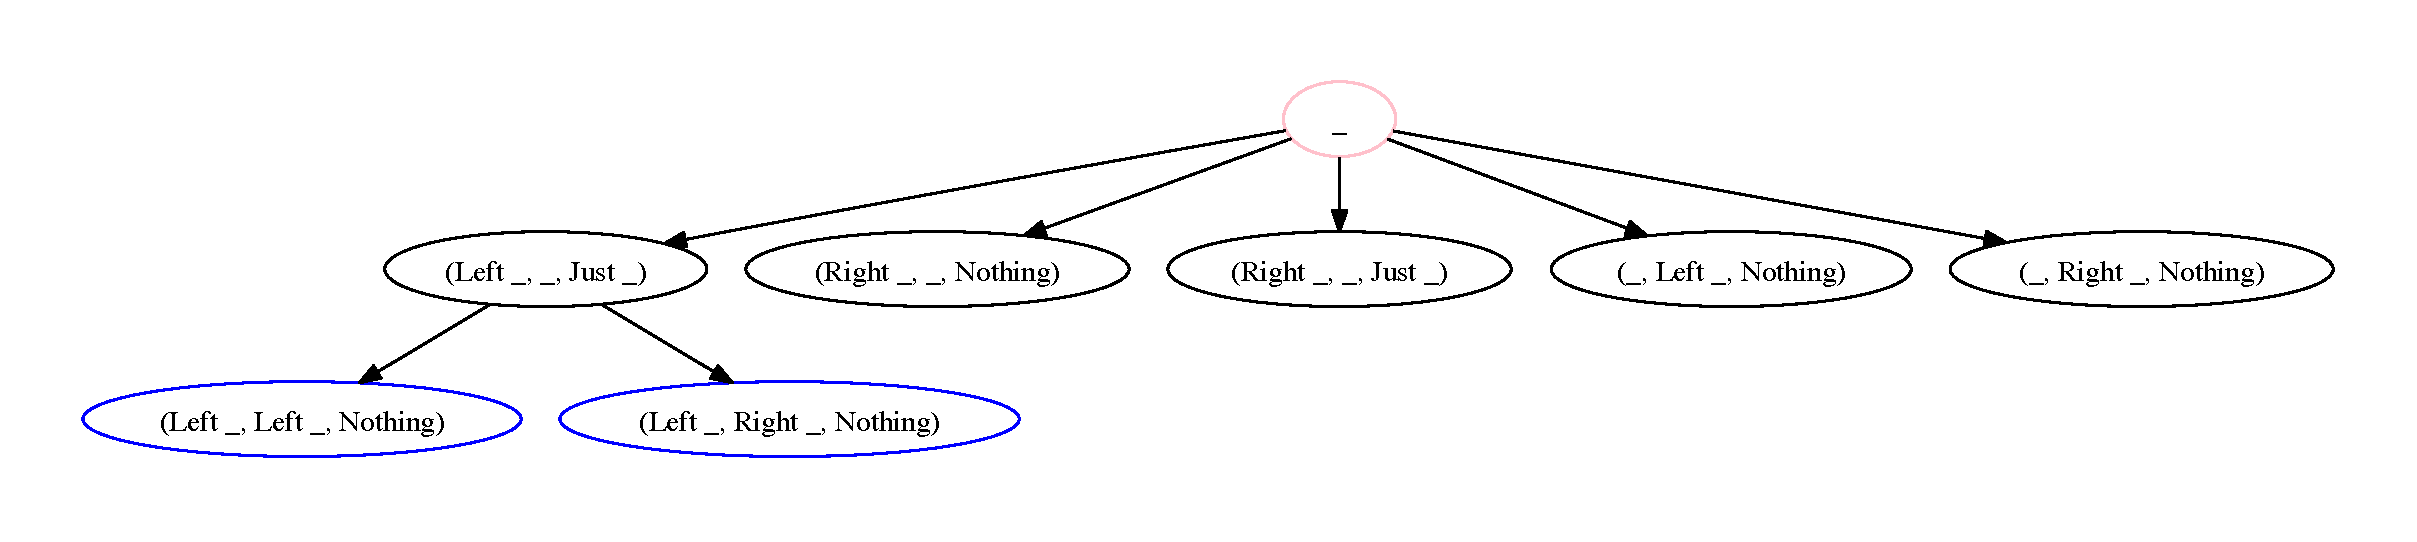
\includegraphics[scale=0.30, trim=10mm 0mm 0mm 10mm, clip]{seeding-2.pdf}
\end{frame}

\begin{frame}{Specialisation graph - 3}
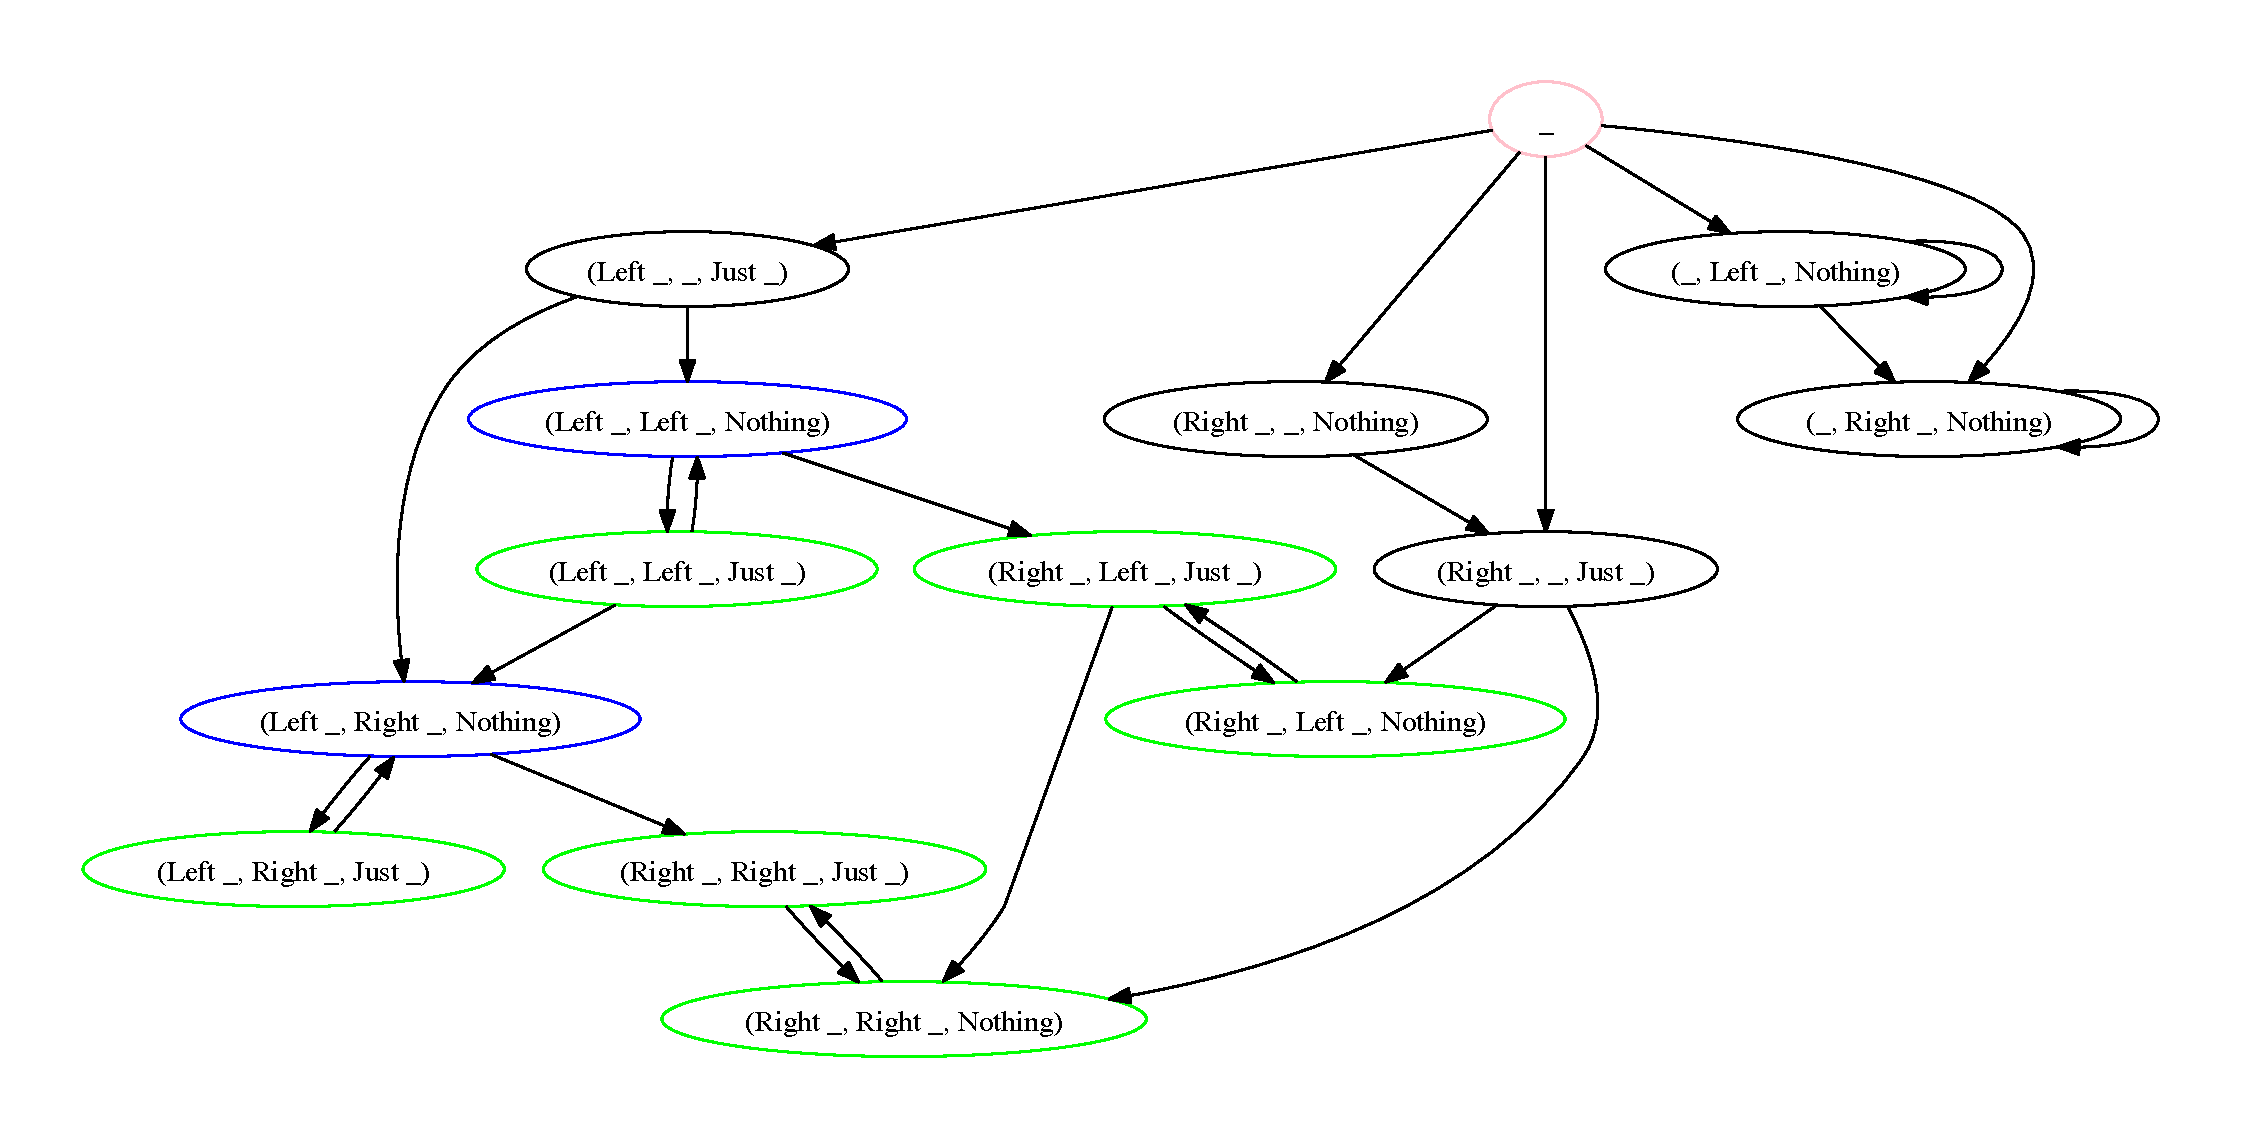
\includegraphics[scale=0.33, trim=10mm 0mm 0mm 10mm, clip]{seeding-3.pdf}
\end{frame}

\begin{frame}[fragile]{Seeding}
\begin{alltt}
main = putStrLn $ show $ go (Left 0, Left 0, Nothing)
\end{alltt}
\end{frame}

\begin{frame}{Seeding of specialisation}
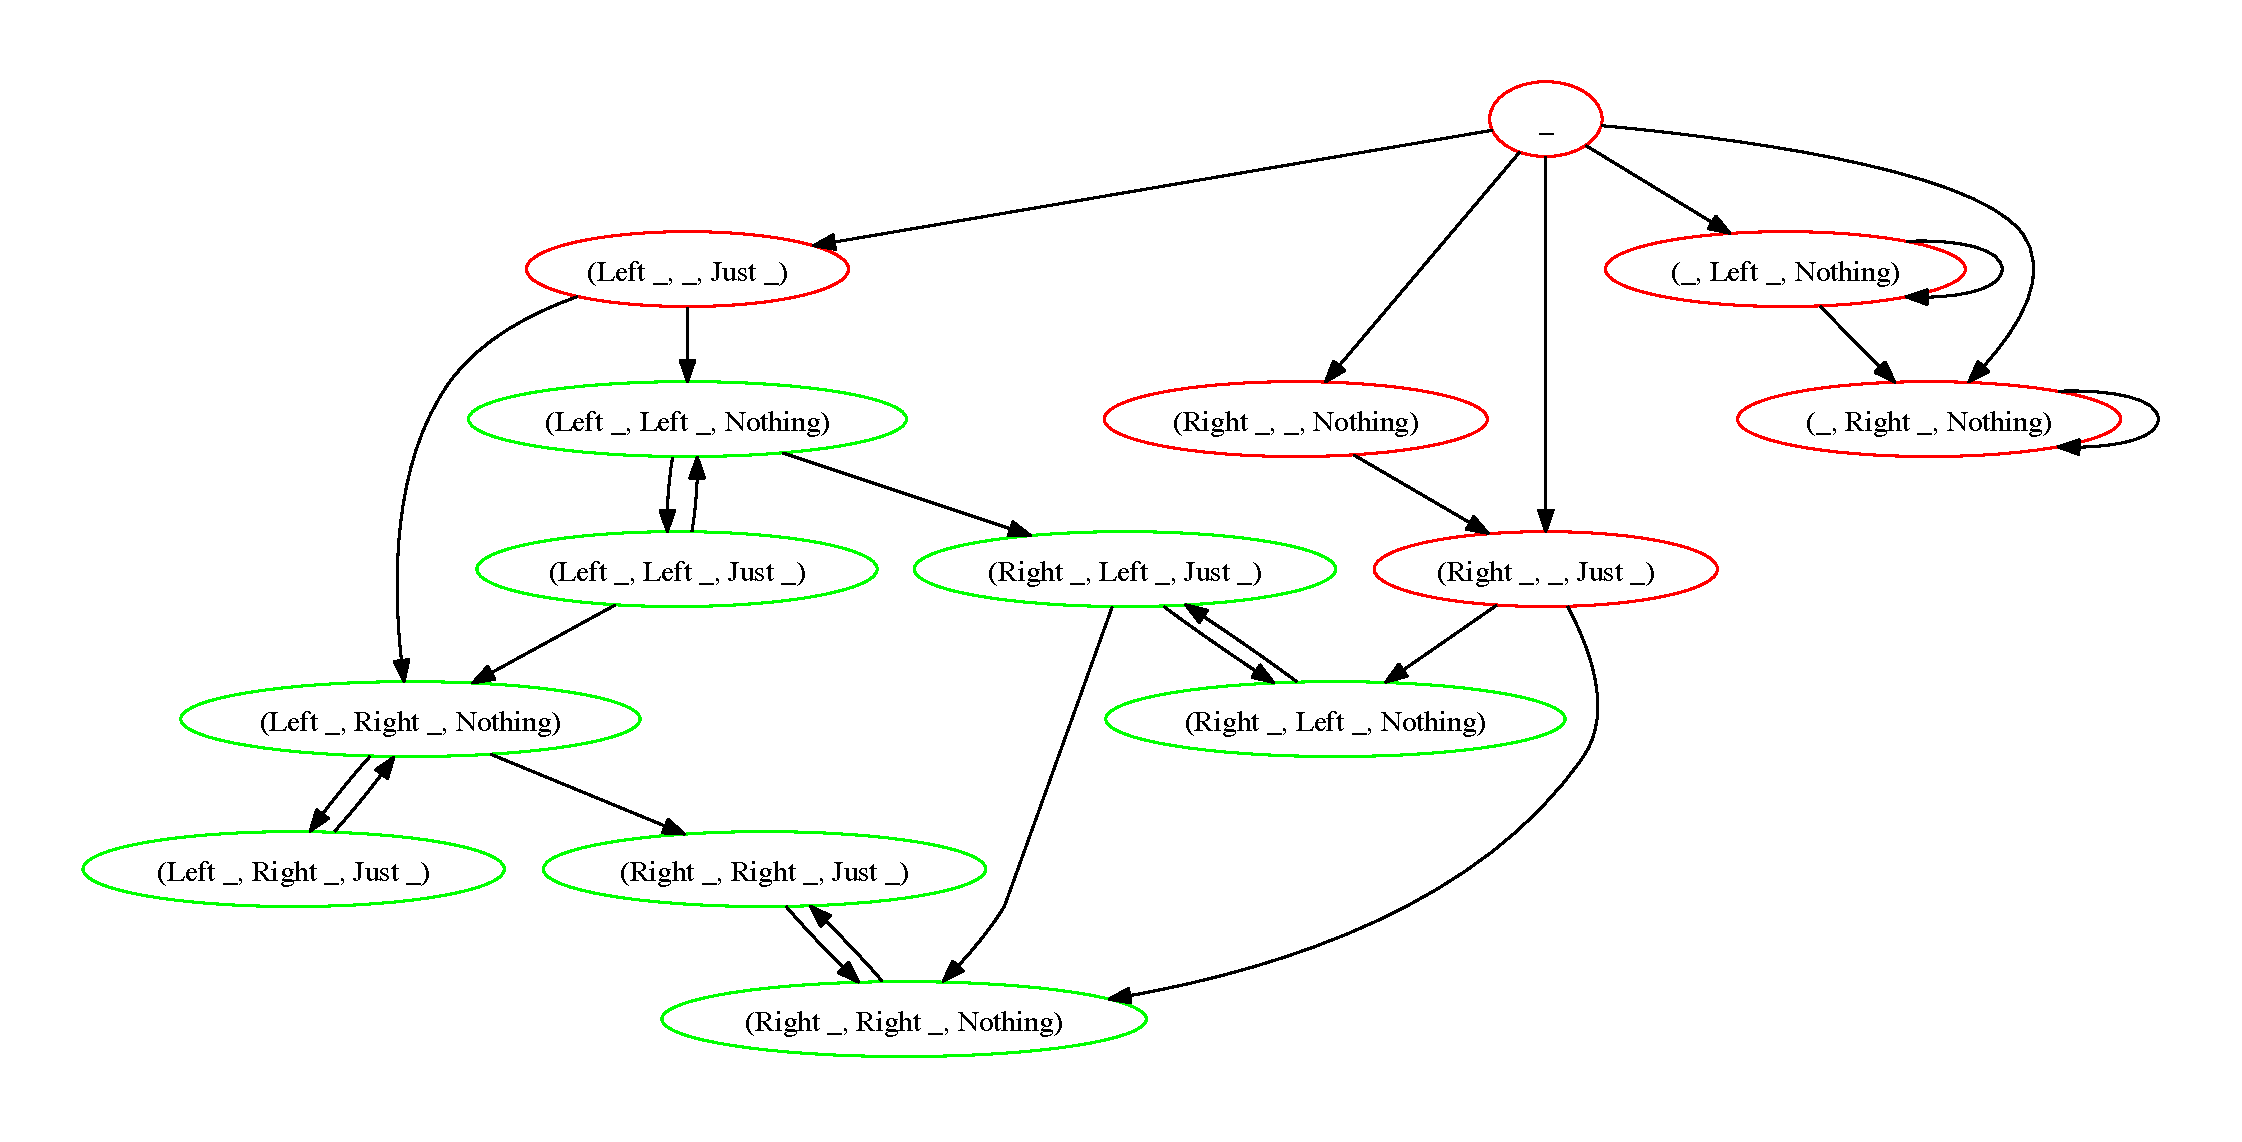
\includegraphics[scale=0.33, trim=10mm 0mm 0mm 10mm, clip]{seeding.pdf}
\end{frame}

\begin{frame}[fragile]{Seeding}
\begin{itemize}
\item Already done for local \verb/let/-defined functions
\item But local \verb/let/ functions can be lifted by simplifier!
\end{itemize}
\end{frame}

\begin{frame}[fragile]{Seeding requirements}
\begin{itemize}
\item Only works if \oomph{go} is not exported
\end{itemize}
Otherwise, calls from other modules could use other call patterns.
\end{frame}

\begin{frame}[fragile]{Seeding requirements}
\begin{itemize}
\item All call patterns must be \emph{interesting}
\end{itemize}
Same as for \verb/let/-defined functions.
\end{frame}



\begin{frame}[fragile]{Code blowup - benchmark}
\begin{alltt}
let xs = enumFromTo 1 len
in       (xs ++ xs) `zip` (xs ++ xs)
   `zip` (xs ++ xs) `zip` (xs ++ xs)
   `zip` (xs ++ xs) `zip` (xs ++ xs)

\oomph{Before}
Result size of SpecConstr
  = {terms: 119,108, types: 415,625, coercions: 9}
(21 seconds)

\oomph{After}
Result size of SpecConstr
  = {terms: 29,372, types: 94,772, coercions: 9}
(3 seconds)
\end{alltt}
\end{frame}



\begin{frame}[fragile]{End}
end.
\end{frame}



\end{document}
